\documentclass[aspectratio=169,fleqn]{beamer}
\usepackage[utf8]{inputenc}

% design
\usetheme{CambridgeUS}
\usecolortheme{beaver}
\setbeamertemplate{itemize items}[square]
\usenavigationsymbolstemplate{\beamertemplatenavigationsymbolsempty}
\definecolor{darkred}{rgb}{0.8,0,0}
\colorlet{grey1}{gray!10!white} % I think = RGB 0.95 0.95 0.95
\colorlet{grey2}{gray!60!white} % I think = RGB 0.7 0.7 0.7
\setbeamercolor{structure}{fg=darkred}
\setbeamertemplate{enumerate item}{\insertenumlabel.}
\setbeamertemplate{itemize item}{$\blacktriangleright$}
\setlength{\tabcolsep}{12pt}
\setbeamercolor{block title}{fg=darkred}

% bibliography
%\usepackage[backend=biber, style=authortitle]{biblatex}
\usepackage{natbib}
\usepackage{har2nat}
\bibliographystyle{unsrt}
%\addbibresource{../../smc.bib}
\usepackage{bibentry}
\nobibliography*

% tikz
\usepackage{tikz}
\usetikzlibrary{positioning}

% maths
\usepackage{amsmath}
\usepackage{amssymb}
\usepackage{amsfonts}
\usepackage{amsthm}
\theoremstyle{definition}
\newtheorem{defn}{Definition}

% useful math symbols
\newcommand{\Prob}{\mathbb{P}}
\newcommand{\PR}{\mathbb{P}}
\newcommand{\E}{\mathbb{E}}
\newcommand{\V}{\operatorname{Var}}
\newcommand{\eqdist}{\overset{d}{=}}
\newcommand{\I}[1]{\mathbb{I}\{#1\}}
\newcommand{\Ntoinfty}{\overset{N\to\infty}{\longrightarrow}}
\newcommand{\limNtoinfty}{\underset{N\to\infty}{\lim}}
\newcommand\indep{\protect\mathpalette{\protect\independenT}{\perp}}
\def\independenT#1#2{\mathrel{\rlap{$#1#2$}\mkern2mu{#1#2}}}

% distributions
\newcommand{\N}{\mathcal{N}}
\newcommand{\Cat}{\operatorname{Categorical}}
\newcommand{\Unif}{\operatorname{Uniform}}
\newcommand{\Mn}{\operatorname{Multinomial}}
\newcommand{\Bin}{\operatorname{Binomial}}

% project-specific commands
\newcommand{\F}{\mathcal{F}_{t-1}}
\newcommand{\vt}[2][t]{\nu_{#1}^{(#2)}}
%\newcommand{\vt}[1]{v_{#1}}
\newcommand{\wt}[2][t]{w_{#1}^{(#2)}}
%\newcommand{\wt}[1]{w_{#1}}
%\newcommand{\wbar}[2][t]{\bar{w}_{#1}^{(#2)}}
%\newcommand{\vttilde}[2][t]{\tilde{v}_{#1}^{(#2)}}
\newcommand{\Et}{\mathbb{E}_{t}}

\title[Non-neutral populations]{Kingman limit for non-neutral populations\\ with applications to sequential Monte Carlo}
\author[Suzie Brown]{\textbf{Suzie Brown} \\[5pt] University of Warwick \\ with Paul Jenkins, Adam Johansen \& Jere Koskela}
\date{22 July 2021} 




\begin{document}

\begin{frame}
	\maketitle
\end{frame}


\begin{frame}{Outline}
	\begin{enumerate}
	\item Kingman's $n$-coalescent \& population models
	\item A history of convergence to the coalescent
	\item Application to sequential Monte Carlo
	\end{enumerate}
\end{frame}


\begin{frame}{Kingman's $n$-coalescent\footnote[frame]{JFC Kingman, \textit{Stochastic Processes \& their Applications}, 1982.}}
	\begin{columns}
	\begin{column}{0.45\textwidth}
		\begin{itemize}
		\item Continuous-time Markov chain on the space of partitions of $\{1,\dots,n\}$
		\item Single pair mergers only
		\item Each pair merges independently at rate 1 (total merge rate $\binom{k}{2}$ while there are $k$ distinct lineages)
		\item Exchangeable
		\end{itemize}
	\end{column}
	\begin{column}{0.45\textwidth}
		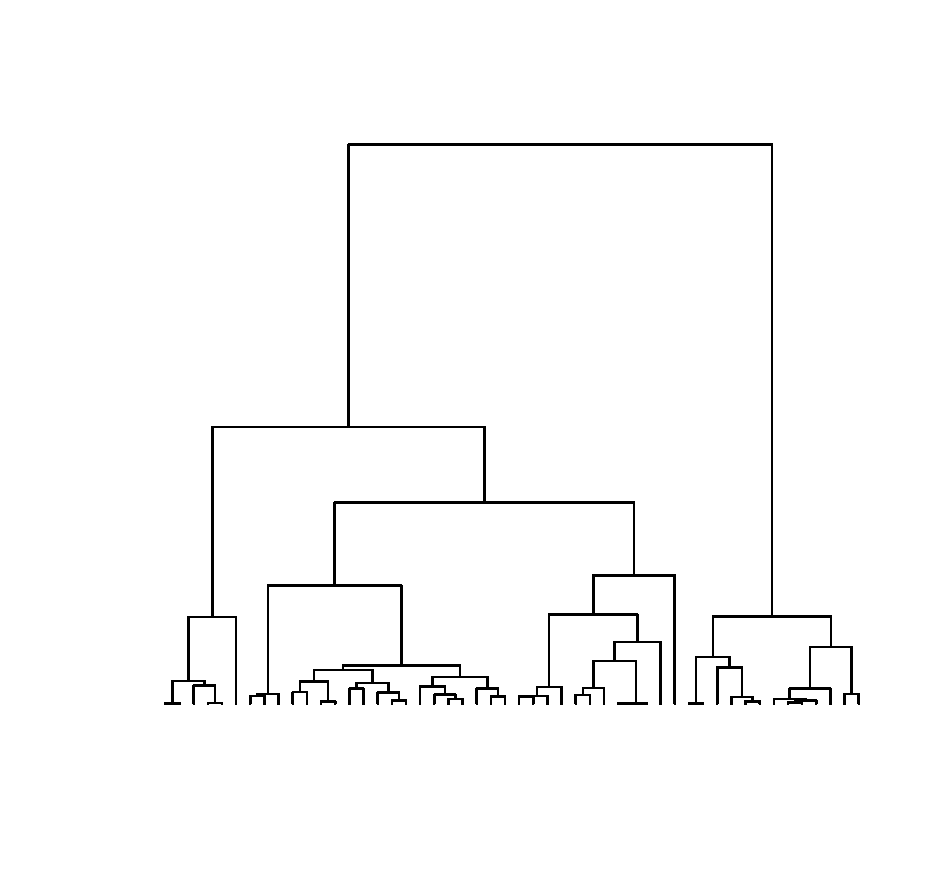
\includegraphics[width=\textwidth, trim={2.8cm 3cm 1.5cm 2cm}, clip]{ncoalescent.pdf}
	\end{column}
	\end{columns}
\end{frame}


\begin{frame}{Question}
    \begin{columns}
    \begin{column}{0.45\textwidth}
	    Under what conditions does a population have genealogies that are asymptotically distributed as $n$-coalescents?
	\end{column}
	\begin{column}{0.45\textwidth}
	    \centering
	    \resizebox{0.8\textwidth}{!}{
		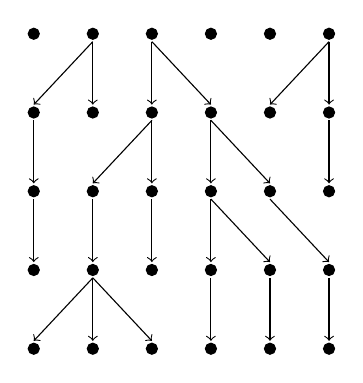
\begin{tikzpicture}
			% grid of particles
			\filldraw (0,0) circle (2pt);
			\filldraw (0.75,0) circle (2pt);
			\filldraw (1.5,0) circle (2pt);
			\filldraw (2.25,0) circle (2pt);
			\filldraw (3,0) circle (2pt);
			\filldraw (3.75,0) circle (2pt);
			\filldraw (0,1) circle (2pt);
			\filldraw (0.75,1) circle (2pt);
			\filldraw (1.5,1) circle (2pt);
			\filldraw (2.25,1) circle (2pt);
			\filldraw (3,1) circle (2pt);
			\filldraw (3.75,1) circle (2pt);
			\filldraw (0,2) circle (2pt);
			\filldraw (0.75,2) circle (2pt);
			\filldraw (1.5,2) circle (2pt);
			\filldraw (2.25,2) circle (2pt);
			\filldraw (3,2) circle (2pt);
			\filldraw (3.75,2) circle (2pt);
			\filldraw (0,3) circle (2pt);
			\filldraw (0.75,3) circle (2pt);
			\filldraw (1.5,3) circle (2pt);
			\filldraw (2.25,3) circle (2pt);
			\filldraw (3,3) circle (2pt);
			\filldraw (3.75,3) circle (2pt);
			\filldraw (0,4) circle (2pt);
			\filldraw (0.75,4) circle (2pt);
			\filldraw (1.5,4) circle (2pt);
			\filldraw (2.25,4) circle (2pt);
			\filldraw (3,4) circle (2pt);
			\filldraw (3.75,4) circle (2pt);
			% resampling arrows % generation 4 to 5
			\draw[->] (0.75,0.9)--(0,0.1);
			\draw[->] (0.75,0.9)--(0.75,0.1);
			\draw[->] (0.75,0.9)--(1.5,0.1);
			\draw[->] (2.25,0.9)--(2.25,0.1);
			\draw[->] (3,0.9)--(3,0.1);
			\draw[->] (3.75,0.9)--(3.75,0.1);
			% resampling arrows % generation 3 to 4
			\draw[->] (0,1.9)--(0,1.1);
			\draw[->] (0.75,1.9)--(0.75,1.1);
			\draw[->] (1.5,1.9)--(1.5,1.1);
			\draw[->] (2.25,1.9)--(2.25,1.1);
			\draw[->] (2.25,1.9)--(3,1.1);
			\draw[->] (3,1.9)--(3.75,1.1);
			% resampling arrows % generation 2 to 3
			\draw[->] (0,2.9)--(0,2.1);
			\draw[->] (1.5,2.9)--(0.75,2.1);
			\draw[->] (1.5,2.9)--(1.5,2.1);
			\draw[->] (2.25,2.9)--(2.25,2.1);
			\draw[->] (2.25,2.9)--(3,2.1);
			\draw[->] (3.75,2.9)--(3.75,2.1);
			% resampling arrows % generation 1 to 2
			\draw[->] (0.75,3.9)--(0,3.1);
			\draw[->] (0.75,3.9)--(0.75,3.1);
			\draw[->] (1.5,3.9)--(1.5,3.1);
			\draw[->] (1.5,3.9)--(2.25,3.1);
			\draw[->] (3.75,3.9)--(3,3.1);
			\draw[->] (3.75,3.9)--(3.75,3.1);
		\end{tikzpicture}
		}
	\end{column}
	\end{columns}
\end{frame}


\begin{frame}{Encoding genealogies}
\begin{columns}
\begin{column}{0.32\textwidth}
\centering
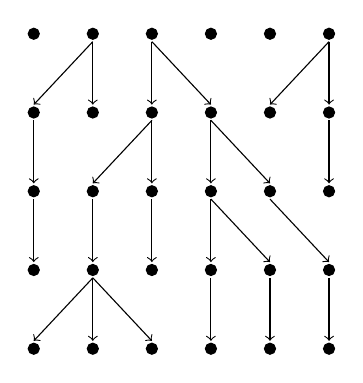
\begin{tikzpicture}
% grid of particles
\filldraw (0,0) circle (2pt);
\filldraw (0.75,0) circle (2pt);
\filldraw (1.5,0) circle (2pt);
\filldraw (2.25,0) circle (2pt);
\filldraw (3,0) circle (2pt);
\filldraw (3.75,0) circle (2pt);
\filldraw (0,1) circle (2pt);
\filldraw (0.75,1) circle (2pt);
\filldraw (1.5,1) circle (2pt);
\filldraw (2.25,1) circle (2pt);
\filldraw (3,1) circle (2pt);
\filldraw (3.75,1) circle (2pt);
\filldraw (0,2) circle (2pt);
\filldraw (0.75,2) circle (2pt);
\filldraw (1.5,2) circle (2pt);
\filldraw (2.25,2) circle (2pt);
\filldraw (3,2) circle (2pt);
\filldraw (3.75,2) circle (2pt);
\filldraw (0,3) circle (2pt);
\filldraw (0.75,3) circle (2pt);
\filldraw (1.5,3) circle (2pt);
\filldraw (2.25,3) circle (2pt);
\filldraw (3,3) circle (2pt);
\filldraw (3.75,3) circle (2pt);
\filldraw (0,4) circle (2pt);
\filldraw (0.75,4) circle (2pt);
\filldraw (1.5,4) circle (2pt);
\filldraw (2.25,4) circle (2pt);
\filldraw (3,4) circle (2pt);
\filldraw (3.75,4) circle (2pt);
% resampling arrows % generation 4 to 5
\draw[->] (0.75,0.9)--(0,0.1);
\draw[->] (0.75,0.9)--(0.75,0.1);
\draw[->] (0.75,0.9)--(1.5,0.1);
\draw[->] (2.25,0.9)--(2.25,0.1);
\draw[->] (3,0.9)--(3,0.1);
\draw[->] (3.75,0.9)--(3.75,0.1);
% resampling arrows % generation 3 to 4
\draw[->] (0,1.9)--(0,1.1);
\draw[->] (0.75,1.9)--(0.75,1.1);
\draw[->] (1.5,1.9)--(1.5,1.1);
\draw[->] (2.25,1.9)--(2.25,1.1);
\draw[->] (2.25,1.9)--(3,1.1);
\draw[->] (3,1.9)--(3.75,1.1);
% resampling arrows % generation 2 to 3
\draw[->] (0,2.9)--(0,2.1);
\draw[->] (1.5,2.9)--(0.75,2.1);
\draw[->] (1.5,2.9)--(1.5,2.1);
\draw[->] (2.25,2.9)--(2.25,2.1);
\draw[->] (2.25,2.9)--(3,2.1);
\draw[->] (3.75,2.9)--(3.75,2.1);
% resampling arrows % generation 1 to 2
\draw[->] (0.75,3.9)--(0,3.1);
\draw[->] (0.75,3.9)--(0.75,3.1);
\draw[->] (1.5,3.9)--(1.5,3.1);
\draw[->] (1.5,3.9)--(2.25,3.1);
\draw[->] (3.75,3.9)--(3,3.1);
\draw[->] (3.75,3.9)--(3.75,3.1);
% fudge bottom space
%\node[anchor=north] at (0,0) {\textcolor{white}{\footnotesize{1}}};
\end{tikzpicture}
\end{column}
\begin{column}{0.62\textwidth}
\centering
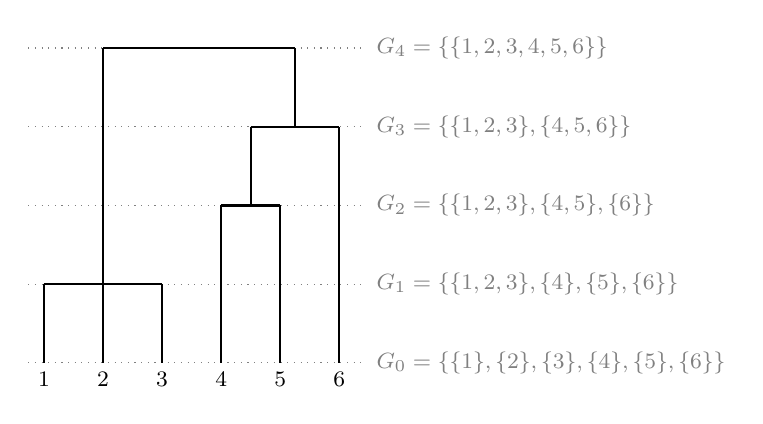
\begin{tikzpicture}
% horizontal time lines
\draw[gray,dotted] (-0.2,0)--(4.05,0);
\draw[gray,dotted] (-0.2,1)--(4.05,1);
\draw[gray,dotted] (-0.2,2)--(4.05,2);
\draw[gray,dotted] (-0.2,3)--(4.05,3);
\draw[gray,dotted] (-0.2,4)--(4.05,4);
% tree
\draw[thick] (0.75,0)--(0.75,4);
\draw[thick] (0,0)--(0,1);
\draw[thick] (1.5,0)--(1.5,1);
\draw[thick] (0,1)--(1.5,1);
\draw[thick] (2.25,0)--(2.25,2);
\draw[thick] (3,0)--(3,2);
\draw[thick] (2.25,2)--(3,2);
\draw[thick] (2.625,2)--(2.625,3);
\draw[thick] (3.75,0)--(3.75,3);
\draw[thick] (2.625,3)--(3.75,3);
\draw[thick] (3.1875,3)--(3.1875,4);
\draw[thick] (0.75,4)--(3.1875,4);
% lineage labels
\node[anchor=north] at (0,0) {\footnotesize{1}};
\node[anchor=north] at (0.75,0) {\footnotesize{2}};
\node[anchor=north] at (1.5,0) {\footnotesize{3}};
\node[anchor=north] at (2.25,0) {\footnotesize{4}};
\node[anchor=north] at (3,0) {\footnotesize{5}};
\node[anchor=north] at (3.75,0) {\footnotesize{6}};
% partition labels
\node[anchor=west] at (4.1,0) {\textcolor{gray}{\footnotesize{$G_0 = \{ \{1\}, \{2\}, \{3\}, \{4\}, \{5\}, \{6\} \}$}}};
\node[anchor=west] at (4.1,1) {\textcolor{gray}{\footnotesize{$G_1 = \{ \{1,2,3\}, \{4\}, \{5\}, \{6\} \}$}}};
\node[anchor=west] at (4.1,2) {\textcolor{gray}{\footnotesize{$G_2 = \{ \{1,2,3\}, \{4,5\}, \{6\} \}$}}};
\node[anchor=west] at (4.1,3) {\textcolor{gray}{\footnotesize{$G_3 = \{ \{1,2,3\}, \{4,5,6\} \}$}}};
\node[anchor=west] at (4.1,4) {\textcolor{gray}{\footnotesize{$G_4 = \{ \{1,2,3,4,5,6\} \}$}}};
\end{tikzpicture}
\end{column}
\end{columns}
\end{frame}


\begin{frame}{Common assumptions on population}
	\begin{itemize}
	\item discrete generations
	\item population size $N(t)$ at generation $t$; define $N:=N(0)$
	\item offspring counts $(\nu_1(t), \dots, \nu_N(t))$ at generation $t$
	\item define the coalescence rate $c_N(t) := \frac{1}{(N)_2} \sum_{i=1}^N (\nu_i(t))_2 $
	%\pause
	\item consider a random sample of $n$ individuals from the terminal generation
	\item scale time to obtain a non-trivial limiting process
	\item take $N\to\infty$
	\end{itemize}
\end{frame}


\begin{frame}{Kingman's sufficient conditions\footnote[frame]{JFC Kingman, \textit{Stochastic Processes \& their Applications}, 1982.}}
    \textbf{Population model:}
	\begin{itemize}
	\item fixed population size $N(t) \equiv N$
	\item offspring counts $(\nu_1(t), \dots, \nu_N(t))$ i.i.d. over $t$
	\item $(\nu_1, \dots, \nu_N)$ exchangeable
	\end{itemize}
	%\pause
	\textbf{Time scale: $N\sigma^{-2}$} \\
	%\pause
	\textbf{Conditions:}
	\begin{itemize}
	\item $\lim_{N\to\infty} \V[\nu_1] = \sigma^2 \in (0,\infty)$
	\item $\E[\nu_1^k] \leq M_k$ for each $k\in\mathbb{N}$
	\end{itemize}
	%\pause
	Then the FDDs of the rescaled sample genealogies converge to those of the $n$-coalescent as $N\to\infty$.
\end{frame}


\begin{frame}{M\"ohle's necessary \& sufficient conditions\footnote[frame]{M M\"ohle, \textit{Advances in Applied Probability}, 2000.}}
    \textbf{Population model:}
	\begin{itemize}
	\item fixed population size $N(t) \equiv N$
	\item offspring counts $(\nu_1(t), \dots, \nu_N(t))$ i.i.d. over $t$
	\item $(\nu_1, \dots, \nu_N)$ exchangeable
	\end{itemize}
	%\pause
	\textbf{Time scale:} 
	\begin{equation*}
	\frac{1}{\E[c_N]} = \frac{N-1}{\V[\nu_1]}
	\end{equation*}
\end{frame}
\addtocounter{footnote}{-1}
\begin{frame}{M\"ohle's necessary \& sufficient conditions\footnote[frame]{M M\"ohle, \textit{Advances in Applied Probability}, 2000.}}
	\textbf{Conditions:}
	\begin{equation*}
	\lim_{N\to\infty} \frac{\E[(\nu_1)_3]}{N\E[(\nu_1)_2]} =0 
	\end{equation*}
	%\pause
	if and only if the FDDs of the rescaled sample genealogies converge to those of the $n$-coalescent as $N\to\infty$.
\end{frame}


\begin{frame}{M\"ohle's sufficient conditions for weak convergence\footnote[frame]{M M\"ohle, \textit{Journal of Applied Probability}, 1998, 1999.}}
    \textbf{Population model:}
    \begin{itemize}
	\item population size $N(t)$ any deterministic function of $t$; $N:=N(0)$
	\item offspring counts $(\nu_1(t), \dots, \nu_N(t))$ independent over $t$
	\item \textit{random assignment condition}: given $(\nu_1(t), \dots, \nu_N(t))$, assignment of offspring to parents is uniform over all valid assignments
	\end{itemize}
	%\pause
	\textbf{Time scale:} some function $\tau_N(t)$ such that for all $t$
	\begin{itemize}
	\item $\lim_{N\to\infty} \sum_{r=1}^{\tau_N(t)} \E[ c_N(r) ] = t$ 
	\item $\lim_{N\to\infty} \sum_{r=1}^{\tau_N(t)} \E[ c_N(r) ]^2 = 0$ 
	\end{itemize}
\end{frame}
\addtocounter{footnote}{-1}
\begin{frame}{M\"ohle's sufficient conditions for weak convergence\footnote[frame]{M M\"ohle, \textit{Journal of Applied Probability}, 1998, 1999.}}
    \textbf{Conditions:} for all $t>0, k\geq 0$
    \begin{equation*}
    \limsup \frac{1}{N(t-1)^3 c_N(t)} \sum_{i=1}^{N(t)} \E[ (\nu_i(t))_2 (\nu_i(t))^k ] =0
    \end{equation*}
    and
    \begin{equation*}
    \limsup \frac{1}{N(t-1)^4 c_N(t)} \sum_{i=1}^{N(t)} \sum_{j=1}^{N(t)} \E[ (\nu_i(t))_2 (\nu_j(t))^2 ] =0 .
    \end{equation*}
    %\pause
    Then the rescaled sample genealogies converge weakly to the $n$-coalescent as $N\to\infty$.
\end{frame}


\begin{frame}{A non-neutral population model}
\centering
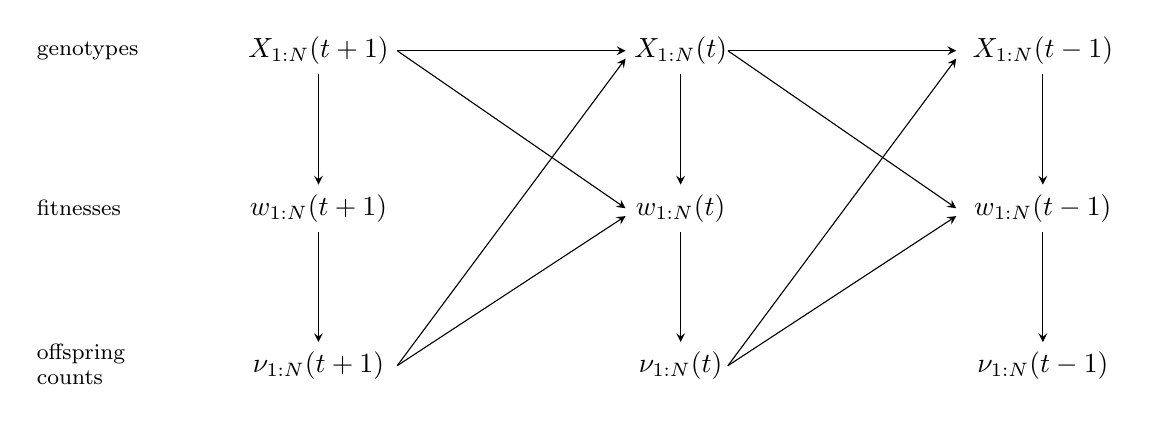
\begin{tikzpicture}[>=stealth]
%% left dots
%\node at (-2,0) {...};
%\node at (-2,-2) {...};
%\node at (-2,-4) {...};
%% labels (t+1)
\node at (-0.5,0) {$X_{1:N}(t+1)$};
\node at (-0.5,-2) {$w_{1:N}(t+1)$};
\node at (-0.5,-4) {$\nu_{1:N}(t+1)$};
%% labels t
\node at (4.1,0) {$X_{1:N}(t)$};
\node at (4.1,-2) {$w_{1:N}(t)$};
\node at (4.1,-4) {$\nu_{1:N}(t)$};
%% labels (t-1)
\node at (8.7,0) {$X_{1:N}(t-1)$};
\node at (8.7,-2) {$w_{1:N}(t-1)$};
\node at (8.7,-4) {$\nu_{1:N}(t-1)$};
%% right dots
%\node at (10,0) {...};
%\node at (10,-2) {...};
%\node at (10,-4) {...};
%% text row labels
\node[anchor=west] at (-4.2,0) {\footnotesize{genotypes}};
\node[anchor=west] at (-4.2,-2) {\footnotesize{fitnesses}};
\node[anchor=west] at (-4.2,-3.85) {\footnotesize{offspring}};
\node[anchor=west] at (-4.2,-4.15) {\footnotesize{counts}};
%
%\pause
%% vertical arrows
\draw[->] (-0.5,-0.3)--(-0.5,-1.7);
\draw[->] (4.1,-0.3)--(4.1,-1.7);
\draw[->] (8.7,-0.3)--(8.7,-1.7);
%
%\pause
%% vertical arrows
\draw[->] (-0.5,-2.3)--(-0.5,-3.7);
\draw[->] (4.1,-2.3)--(4.1,-3.7);
\draw[->] (8.7,-2.3)--(8.7,-3.7);
%
%\pause
%% arrows
\draw[->] (0.5,0)--(3.4,0);
\draw[->] (4.7,0)--(7.6,0);
\draw[->] (0.5,-4)--(3.4,-0.1);
\draw[->] (4.7,-4)--(7.6,-0.1);
%
%\pause
%% arrows
\draw[->] (0.5,0)--(3.4,-2);
\draw[->] (0.5,-4)--(3.4,-2.1);
\draw[->] (4.7,0)--(7.6,-2);
\draw[->] (4.7,-4)--(7.6,-2.1);
\end{tikzpicture}
\end{frame}


%\begin{frame}{Koskela et al's sufficient conditions\footnote[frame]{J Koskela, PA Jenkins, AM Johansen, D Span\`o, \textit{The Annals of Statistics}, 2020.}}
%	...\\
%	\textbf{Conditions:}
%	\begin{itemize}
%	\item 
%	\end{itemize}
%\end{frame}

\begin{frame}{Sufficient conditions for weak convergence\footnote[frame]{S Brown, PA Jenkins, AM Johansen, J Koskela, \textit{Electronic Journal of Probability}, 2021.}}
	\textbf{Population model:}
	\begin{itemize}
		\item fixed population size $N(t) \equiv N$
		\item offspring counts $(\nu_1(t), \dots, \nu_N(t))$ conditionally dependent over $t$ as in previous slide
		\item random assignment condition
	\end{itemize}
	\textbf{Time scale:}
	\begin{equation*}
	\tau_N(t) := \min \left\{ s: \sum_{r=1}^s c_N(r) \geq t \right\}
	\end{equation*}
	and assume that $\Prob[\tau_N(t) = \infty] =0$ for all finite $t$ 
\end{frame}
\addtocounter{footnote}{-1}
\begin{frame}{Sufficient conditions for weak convergence\footnote[frame]{S Brown, PA Jenkins, AM Johansen, J Koskela, \textit{Electronic Journal of Probability}, 2021.}}
	\textbf{Conditions:} there exists a deterministic sequence $b_N \to 0$ such that for all $N,t$
	\begin{equation*}
	\frac{1}{N} \sum_{i=1}^N \Et[ (\nu_i(t))_3 ] \leq b_N  \sum_{i=1}^N \Et[ (\nu_i(t))_2 ]
	\end{equation*}
	%\pause
	Then the rescaled sample genealogies converge weakly to the $n$-coalescent as $N\to\infty$.
\end{frame}


\begin{frame}{Sequential Monte Carlo}
	\textbf{Aim:} simulate a particle system that approximates a given sequence of probability distributions.\\
	\vspace{10pt}
	
	%\pause
	Initialise $N$ particles by sampling their genotypes $X_{1:N}$ from some distribution $\mu(\cdot)$\\[5pt]
	
	Then iterate these steps:
	\begin{enumerate}
	\item \textbf{(mutation)} update the genotypes via Markov kernel $M_t$
	\item \textbf{(fitness)} calculate fitness scores by applying function $g_t$ to the genotypes
	\item \textbf{(selection)} resample particles according to their fitnesses
	\end{enumerate}
	\vspace{10pt}
	
	%\pause
	\begin{itemize}
	\item $\mu$, $(M_t)$ and $(g_t)$ are chosen such that the particle system approximates the desired distributions
	\item The selection step induces a genealogy, which affects performance of the algorithm
	\end{itemize}
\end{frame}


\begin{frame}{Sequential Monte Carlo genealogies}
	\begin{itemize}
	\item Most of the popular sequential Monte Carlo algorithms have asymptotically Kingman genealogies\footnote{S Brown, PA Jenkins, AM Johansen, J Koskela, \textit{Electronic Journal of Probability}, 2021.}
	\item The time scale differs depending on the particular algorithm, and is an indicator of performance 
	\item Explicitly characterising the time scale would allow better tuning and comparisons between algorithms
	\end{itemize}
\end{frame}


\begin{frame}{In conclusion...}
\begin{itemize}
\item Many neutral population models are known to have asymptotically Kingman genealogies
\item We add to these a large class of non-neutral models, having a particular conditional independence structure rather than independent generations
\item For these models, weak convergence to the $n$-coalescent is proved under simple sufficient conditions
\item This result is applied to several popular sequential Monte Carlo algorithms
\item The next step is to describe explicitly the time scale function in these cases
\end{itemize}
\end{frame}


\begin{frame}{References}
\begin{description}
\item [1,2] JFC Kingman (1982) \textit{On the genealogy of large populations}, Stochastic Processes and their Applications.
\item [3] M M\"ohle (2000) \textit{Total variation distances and rates of convergence for ancestral coalescent processes in exchangeable population models}, Advances in Applied Probability.
\item [4a] M M\"ohle (1998) \textit{Robustness results for the coalescent}, Journal of Applied Probability.
\item [4b] M M\"ohle (1999) \textit{Weak convergence to the coalescent in neutral population models}, Journal of Applied Probability.
\item [5,6] S Brown, PA Jenkins, AM Johansen, J Koskela (2021) \textit{Simple conditions for convergence of sequential Monte Carlo genealogies with applications}, Electronic Journal of Probability.
\end{description}
\end{frame}

\end{document}